\documentclass{article}

\usepackage{graphicx} %package to manage images
\usepackage{subfigure}
\usepackage{wrapfig}
\graphicspath{  {./figures/}  }

% if you need to pass options to natbib, use, e.g.:
%     \PassOptionsToPackage{numbers, compress}{natbib}
% before loading neurips_2021

% ready for submission
\usepackage[preprint]{neurips_2021}

% to compile a preprint version, e.g., for submission to arXiv, add add the
% [preprint] option:
%     \usepackage[preprint]{neurips_2021}

% to compile a camera-ready version, add the [final] option, e.g.:
%     \usepackage[final]{neurips_2021}

% to avoid loading the natbib package, add option nonatbib:
%    \usepackage[nonatbib]{neurips_2021}

\usepackage[utf8]{inputenc} % allow utf-8 input
\usepackage[T1]{fontenc}    % use 8-bit T1 fonts
\usepackage{hyperref}       % hyperlinks
\usepackage{url}            % simple URL typesetting
\usepackage{booktabs}       % professional-quality tables
\usepackage{amsfonts}       % blackboard math symbols
\usepackage{nicefrac}       % compact symbols for 1/2, etc.
\usepackage{microtype}      % microtypography
\usepackage{xcolor}         % colors

\title{Analysis and Visualization of\\ Data Scientist Salaries}

% The \author macro works with any number of authors. There are two commands
% used to separate the names and addresses of multiple authors: \And and \AND.
%
% Using \And between authors leaves it to LaTeX to determine where to break the
% lines. Using \AND forces a line break at that point. So, if LaTeX puts 3 of 4
% authors names on the first line, and the last on the second line, try using
% \AND instead of \And before the third author name.

\author{%
  Sithara Aysha\\
  University of Tübingen\\ 
  M.Sc. Quantitative Data Science Methods in Psychometrics, Econometrics and Machine Learning\\
  \And
  Christina Müller\\
   University of Tübingen\\
   M.Sc. Quantitative Data Science Methods in Psychometrics, Econometrics and Machine Learning \\
  % examples of more authors
  % \And
  % Coauthor \\
  % Affiliation \\
  % Address \\
  % \texttt{email} \\
  % \AND
  % Coauthor \\
  % Affiliation \\
  % Address \\
  % \texttt{email} \\
  % \And
  % Coauthor \\
  % Affiliation \\
  % Address \\
  % \texttt{email} \\
  % \And
  % Coauthor \\
  % Affiliation \\
  % Address \\
  % \texttt{email} \\
}

\begin{document}

\maketitle

\begin{abstract}
    We use a data set containing \href{https://www.kaggle.com/jackogozaly/data-science-and-stem-salaries}{2,578 Data Scientists salary records from top companies} originally sourced from \href{https://www.levels.fyi}{levels.fyi}. We analyse how much Data Scientists earn with respect to their experience, gender, ethnicity and education. Furthermore, different visualizations regarding which companies or locations offer better packages to Data Scientists are made. Exploratory analysis methods and visualization tools like choropleth maps are used. \\
    Link Git repository: \href{https://github.com/sitharaayesha/DataScientistsSalaries.git}{https://github.com/sitharaayesha/DataScientistsSalaries.git}
\end{abstract}

\section{Introduction}

In 2012 Harvard Business Magazine titled Data Scientist the sexiest job of the 21st century (Davenport and Patil, 2012). More and more people are working as Data Scientists in companies worldwide. In this report, a data set with information of about 2,578 Data Scientists salaries is being analyzed with respect to their working location, experience, gender, ethnicity and education.

\section{Data}
The original data set contains 62,642 samples and 29 features, which include ‘company', ‘title', ‘totalyearlycompensation', ‘location', ‘yearsofexperience', ‘gender', ‘race', and ‘education' to name a few. We subset the data to include only information on Data Scientists and clean the data. 
Outliers with extreme values of the yearly salaries have been removed as we stick with samples between the fifth and ninety fifth percentile. As the salary is of main interest in this report, we are taking total yearly compensation as the basis for all analysis and are treating it as the dependent variable in the statistical analysis. After data cleaning the data set shows a mean total yearly compensation of \$194,972 and a median compensation of \$185,000. The 25\% quantile is \$140,000 and the 75\% quantile \$240,000. The lowest total yearly compensation of a Data Scientist in our sample is \$70,000 and the highest \$400,000 (figure \ref{fig:distribution}).

 \begin{figure}
    \centering
    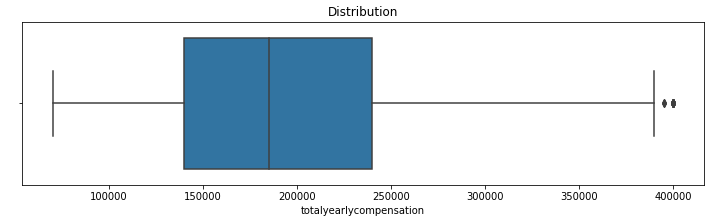
\includegraphics[width=0.7\linewidth]{NeurIPS_style/figures/Distribution.png}
    \caption{Distribution of Total Yearly Compensation of Data Scientists}
    \label{fig:distribution}
\end{figure}

\section{Visualizations}
As the first step, we check the differences in salaries paid by different companies. The companies providing the highest total yearly compensations on average are the hedge fund company Citadel, the communications technology company Zoom and the investment bank JP Morgan, all of which pay at least \$400,000 a year (figure \ref{fig:basic_visualization_a}). Even though these companies are the ones paying the highest compensations, the top five companies hiring Data Scientists in absolute numbers are Amazon, Microsoft, Facebook, Google and Apple (figure \ref{fig:basic_visualization_b}), all of which are data-driven companies and belong to the top ten companies ranked by Market capitalization.

\begin{figure}
    \subfigure[]{
    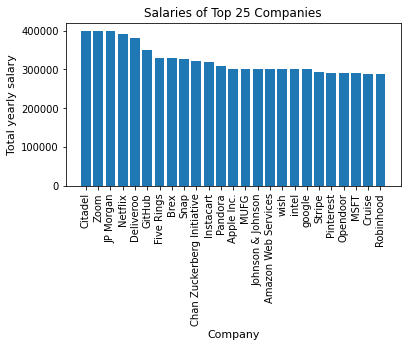
\includegraphics[width=0.5\linewidth]{Salaries of Top 25 Companies}   
    \label{fig:basic_visualization_a}
    }
    \subfigure[]{
    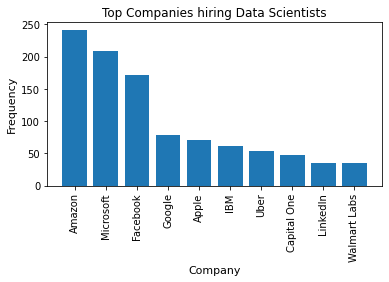
\includegraphics[width=0.6\linewidth]{Top Companies hiring Data Scientists}
    \label{fig:basic_visualization_b}
    }
    \subfigure[]{
    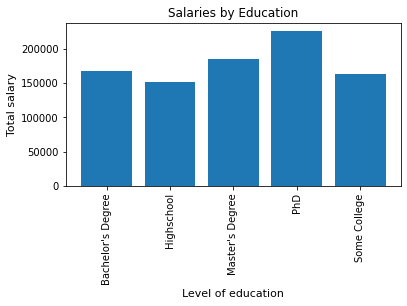
\includegraphics[width=0.55\linewidth]{Salaries by Education}
    \label{fig:basic_visualization_c}
    }
    \subfigure[]{
    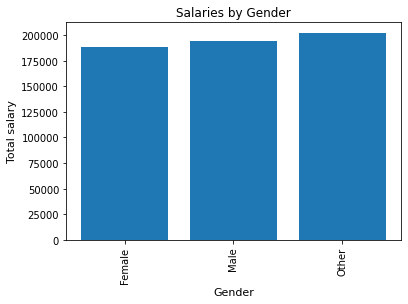
\includegraphics[width=0.55\linewidth]{Salaries by Gender}
    \label{fig:basic_visualization_d}
    }
    \caption{Exploratory Analysis}
    \label{fig:basic_visualization}
\end{figure}

Furthermore, salaries are compared with respect to education and degree qualifications (figure \ref{fig:basic_visualization_c}). It does not come as a surprise that higher the degree qualification, higher the mean total yearly compensation. Data Scientists with a PhD earn the most money. The category ‘some college' has not been defined in the data set, but professionals with that form of education earn on average similar to Data Scientists holding a Bachelor's degree.

Lastly, we look at the difference in salaries between genders (figure \ref{fig:basic_visualization_d}). The mean total yearly compensation of men is slightly higher than that of women. Those who identify as ‘other' have an even higher income. It is worth noticing that nearly one third of the Data Scientists in the data set did not give any information about their gender. 

Additionally, the mean salaries in the different US states and countries are visualized in separate choropleths. As it is still quite a small data set, several US states and countries do not contain any data. They are denoted by a light grey color. The US map (figure \ref{fig:US_map}) shows that Data Scientists working in the neighbor states Missouri, Kansas and Oklahoma get the highest yearly income. Particularly low financial compensations for Data Scientists are observed in Utah, Indiana, Kentucky, Tennessee and Mississippi.

\begin{figure}
    \centering
    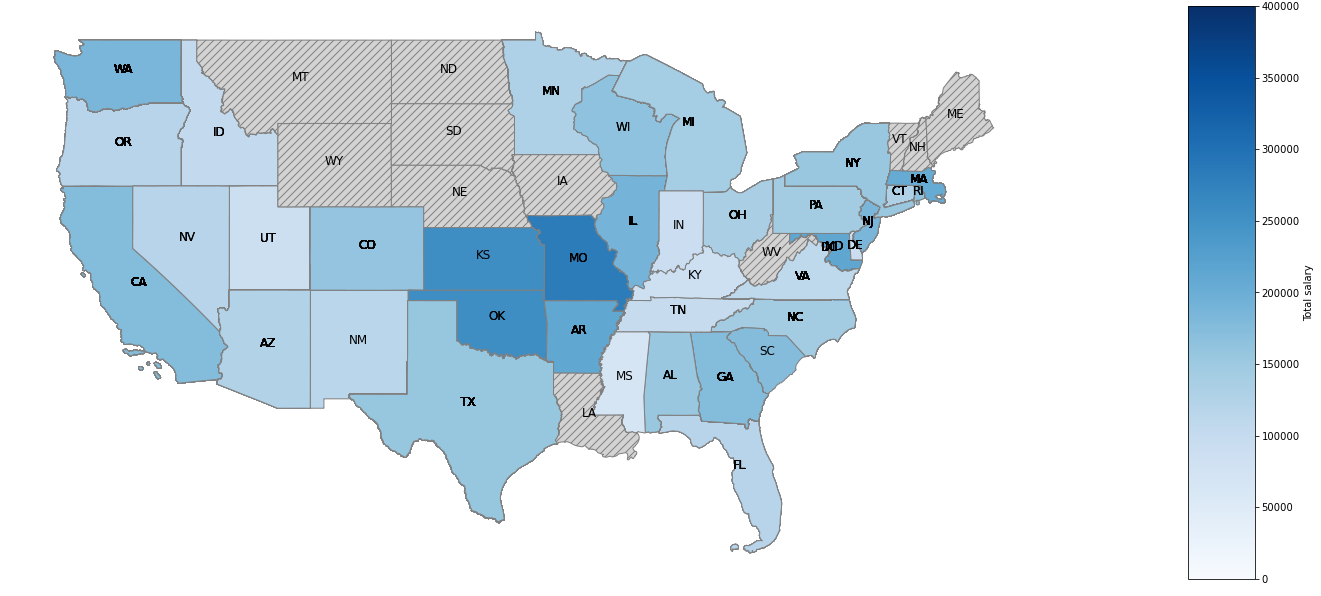
\includegraphics[width=1.05\linewidth]{NeurIPS_style/figures/usa_map.png}
    \caption{Data Scientist Salaries in the USA}
    \label{fig:US_map}
\end{figure}
 

Looking at the world map (figure \ref{fig:world_map}), we can see that Data Scientists in the United States of America, as well as in Israel and France have the highest mean total yearly compensation. On the other hand, Ukraine and Luxembourg have the lowest income. Hong Kong and Singapore are not shown in the plot as there is no geodata available. Hong Kong has the second highest mean yearly compensation, Singapore the ninth highest.

\begin{figure}
    \centering
    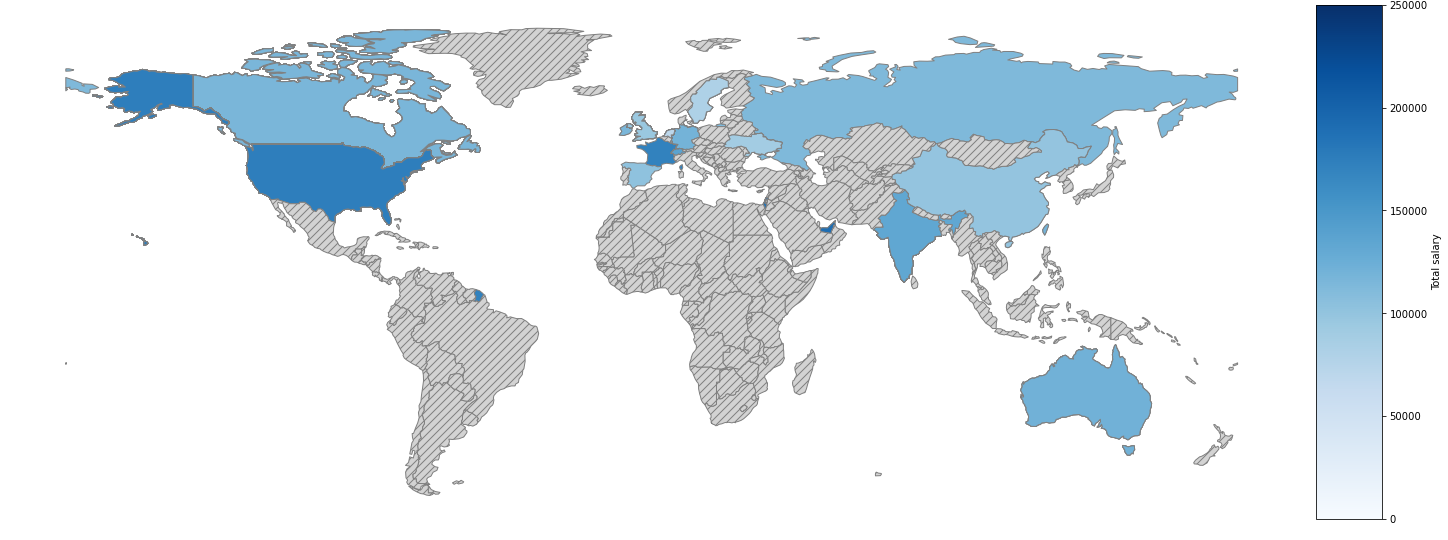
\includegraphics[width=1.05\linewidth]{NeurIPS_style/figures/world_map.png}
    \caption{Data Scientist Salaries throughout the World}
    \label{fig:world_map}
\end{figure}

\section{Statistical Analysis}
We use regressive models to analyse the relationship between the salary (target variable) and explanatory variables such as the company, gender, years of experience, etc. We want to know which factors have high correlation with growing salaries. Then the salary can be predicted based on the values of these explanatory covariates.

The categorical variables are label encoded for regression, and a smaller subset out of the 29 covariates are taken into consideration. The correlation plot of the design matrix confirms that no chosen covariates provide redundant information. Our data is randomly split into training and test set (25\%). The models are trained on the training set and their performance is evaluated based on their salary predictions on the unseen test set. We use the Root Mean Square Error, Cross Validation Score, and R-squared values as metrics for model evaluation. 

\subsection{Linear Regression}
In linear regression models, a linear relationship between the dependent and independent variables are assumed. LinearRegression function from the Scikit-learn library is used to build the model. The training set is fit to the model, and the linear model is used to predict the salary of test data. We notice that the model fits the data fairly well with R-squared value of 0.94, RMSE of 16798.85 and CV Score of 17078.04. This indicates a linear relationship between yearly salary and variables like gender, education, and years of experience.


\subsection{Random Forest}
Random decision forest builds many decision trees on random samples of data using bootstrap aggregating, and takes their average as the result. RandomForestRegressor function from the Scikit-learn library is used to build the model. Our Random forest model has R-squared value of 0.95, RMSE of 15889.23 and CV Score of 18975.94.



\subsection{XGBoost}
To further improve our salary predictions, we build an Extreme Gradient Boosting (XGBoost) model using the xgboost library. This model makes use of gradient boosted decision trees. Gradient descent algorithm is used to add models sequentially to improve on current errors, until no more improvements can be made. Similar to the Random forest model, the parameters ‘basesalary', ‘stockgrantvalue', and ‘bonus' are given higher feature importance. The model has R-squared value of 0.94, RMSE of 16429.77 and CV Score of 18191.32.



\section{Conclusion}
All in all, we have observed some interesting analytic results and visualisations. We built some regressive models to predict Data Scientist salaries based on selected independent variables. According to the given data, we can say that the salary increases with years of experience, education, and there also seems to be a pay gap between genders.

As the data set is quite small, more extensive data on Data Scientist salaries would give further insight in salaries, as well as possible differences with respect to gender, location, ethnicity and education.

\section*{References}

{
\small

 [1] Davenport,Thomas H. \ \&  Patil, D.J. \ (2012) Data scientist: The sexiest job of the 21st Century. Harvard Business Review. Available at: https://hbr.org/2012/10/data-scientist-the-sexiest-job-of-the-21st-century [Accessed January 26, 2022].}
 


\end{document}